\section{Reference Model}
\begin{frame}\frametitle{Reference Model}
	\begin{itemize}
		\item Single Model
	\end{itemize}
	\begin{itemize}
		\item Abstract
		\item Flexibility
		\begin{itemize}
			\item Allow changes if needed
		\end{itemize}
	\end{itemize}
\end{frame}
\begin{frame}\frametitle{Reference Model}
	\begin{figure}
		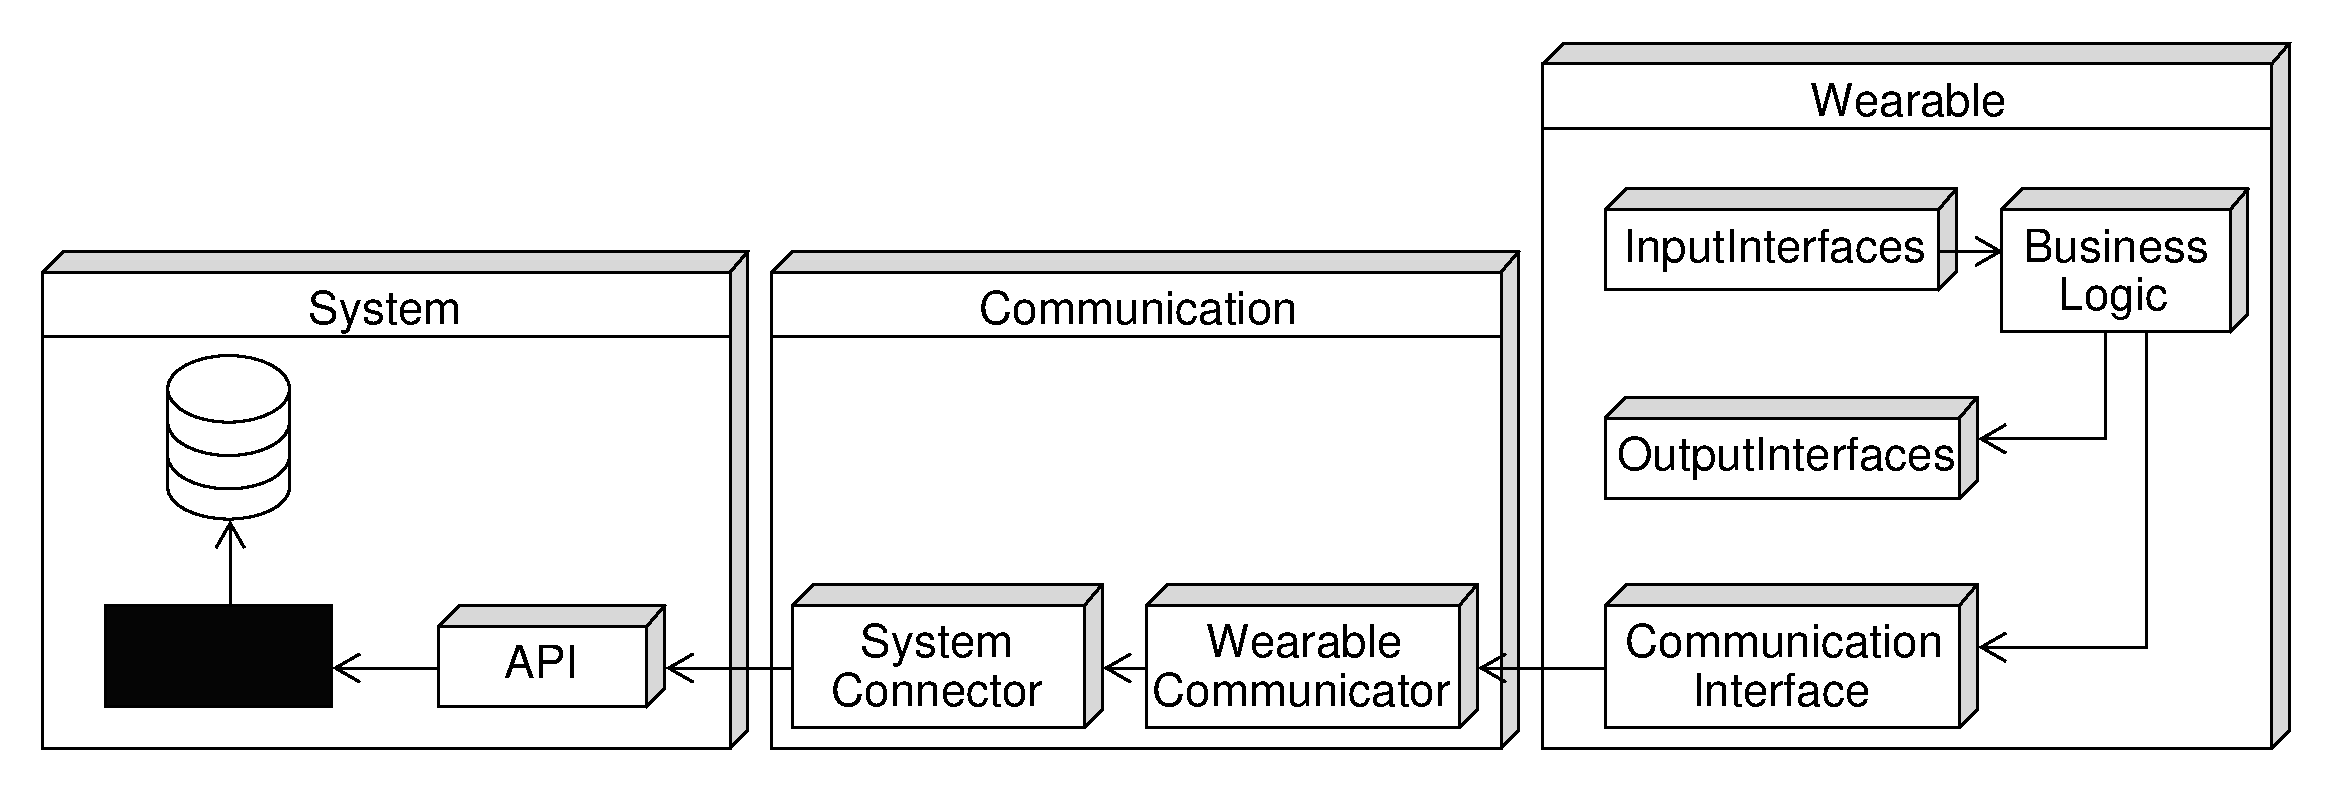
\includegraphics[width=\textwidth]{images/ReferenceModel}
	\end{figure}
\end{frame}
\begin{frame}\frametitle{Reference Model Examples}
	\begin{figure}
		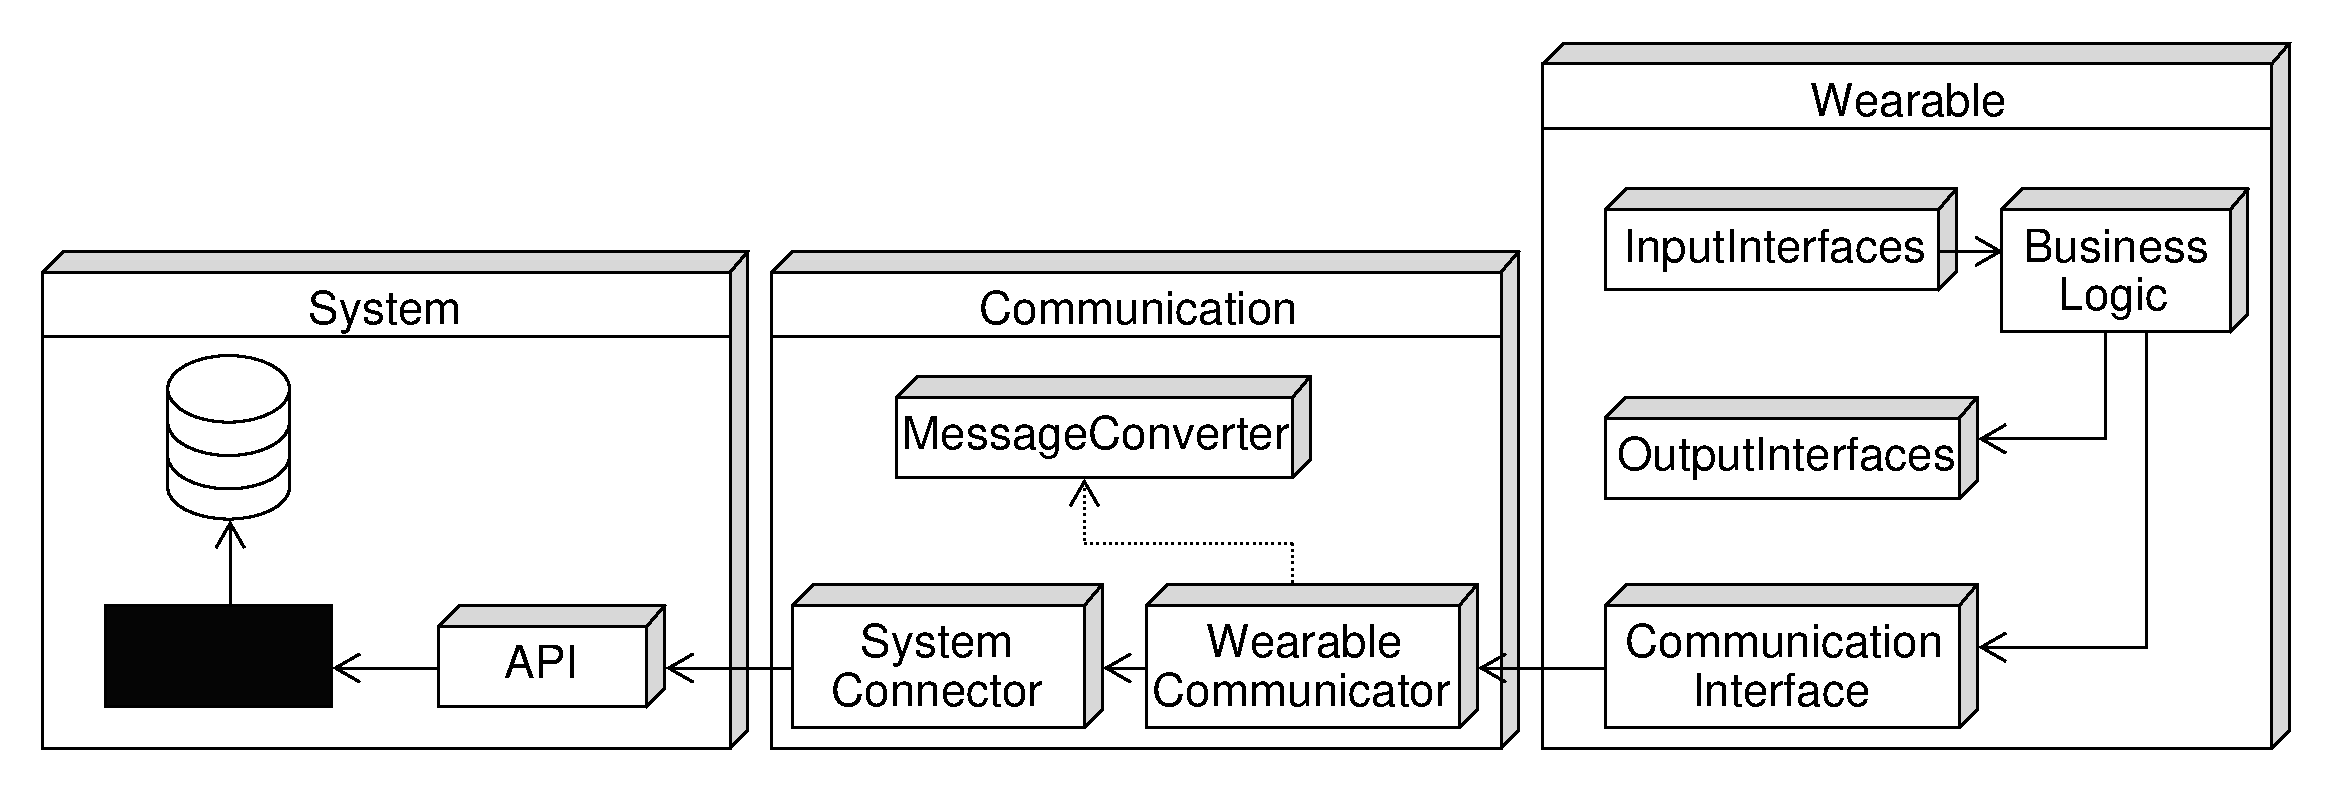
\includegraphics[width=\textwidth]{images/ReferenceModel_Converter}
	\end{figure}
\end{frame}
\begin{frame}\frametitle{Reference Model Examples}
	\begin{figure}
		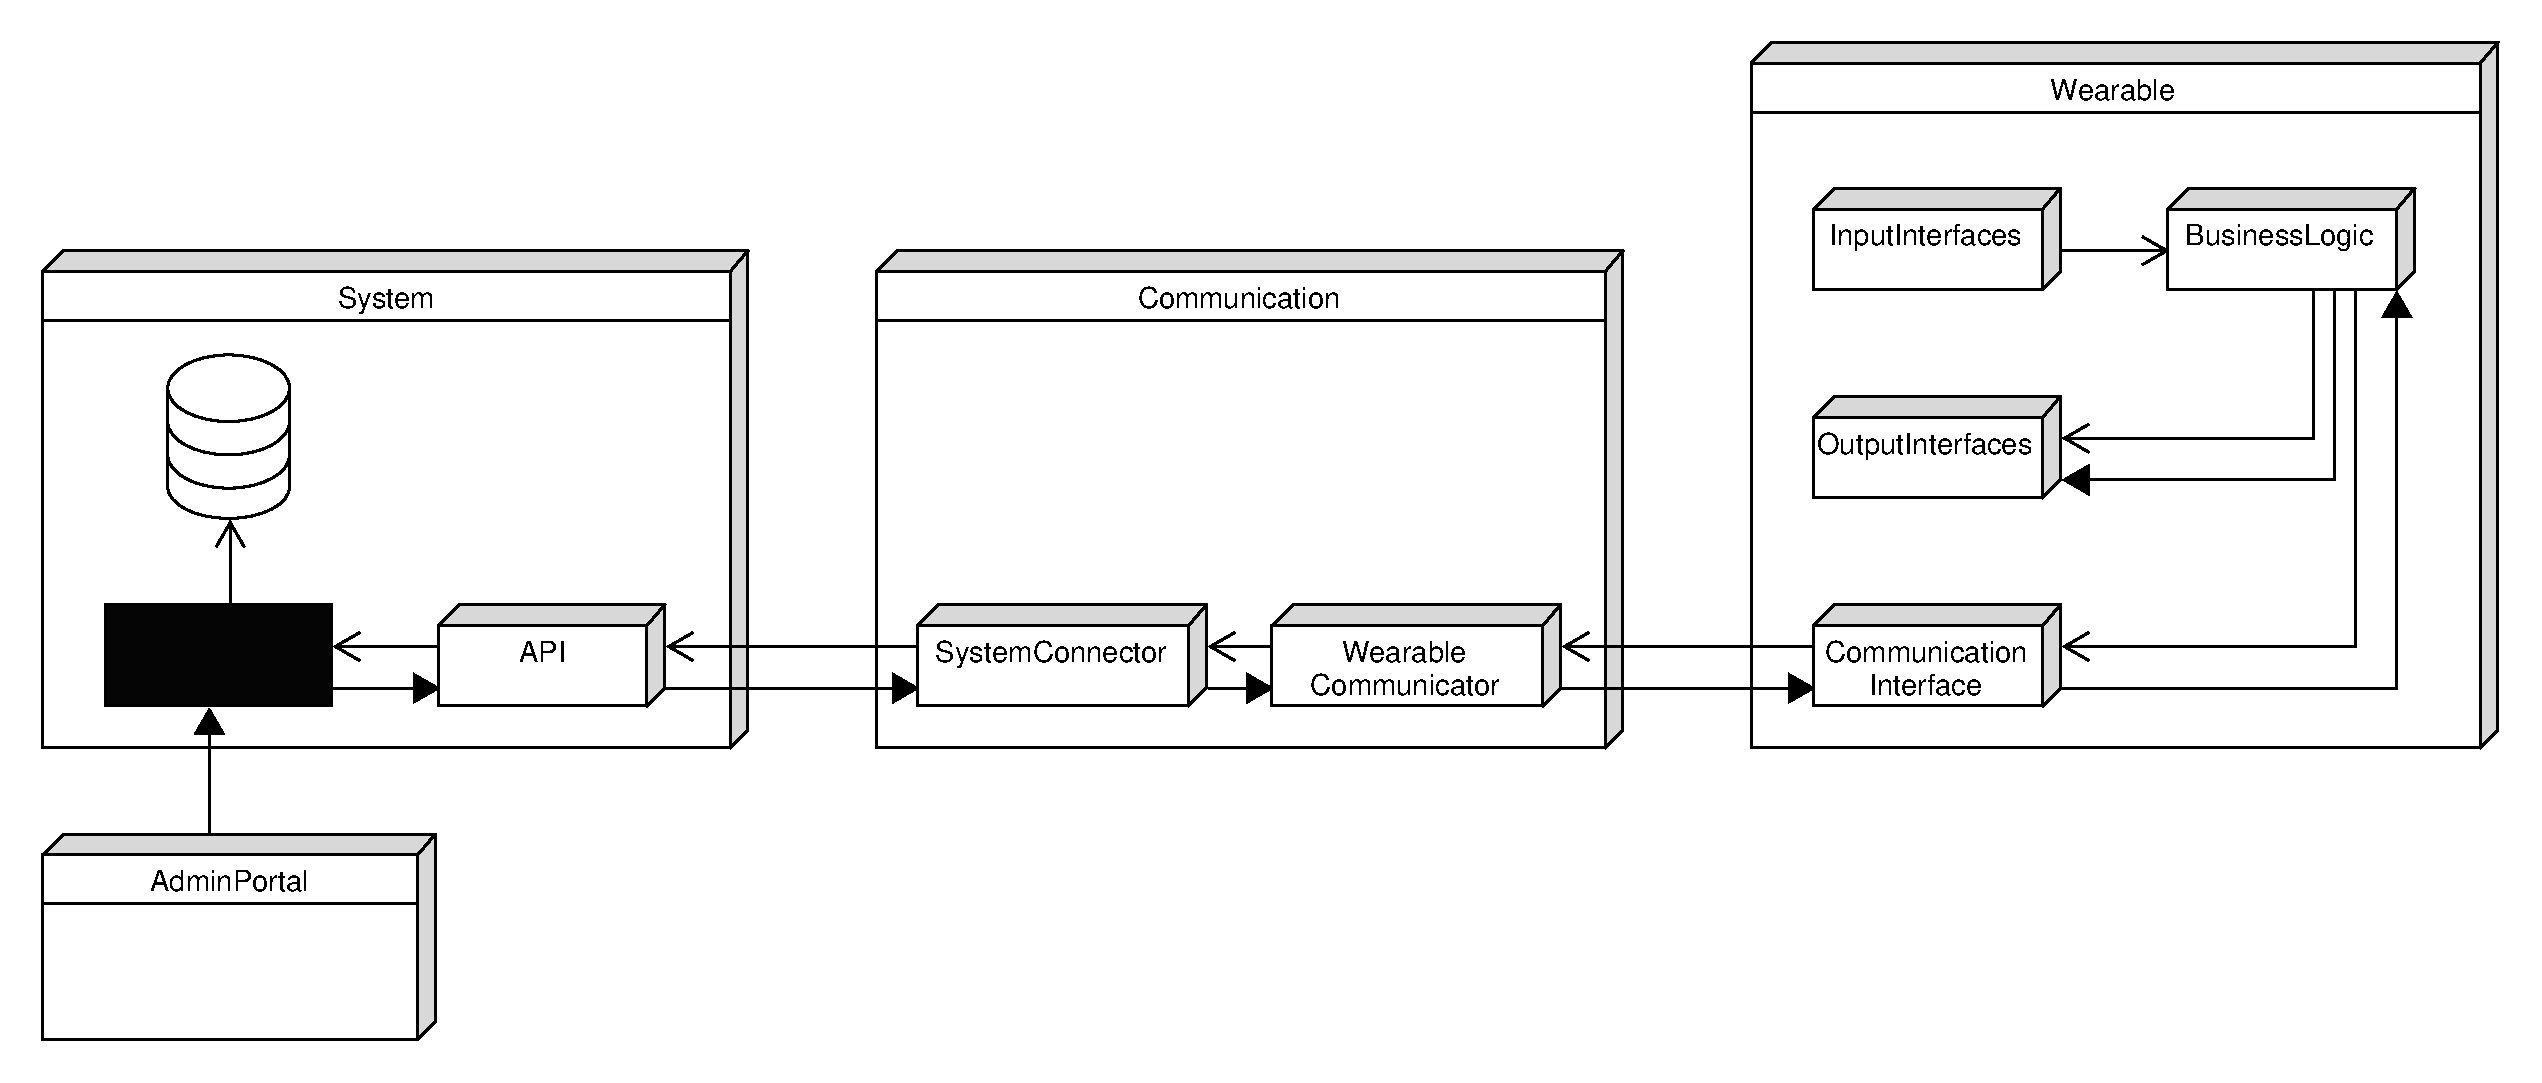
\includegraphics[width=\textwidth]{images/PackageModel_ReferenceArchitecture_PushMessages}
	\end{figure}
\end{frame}
